\documentclass[a4paper,10pt]{article}
\usepackage[utf8]{inputenc}
\usepackage[hyphens]{url}
\usepackage{graphicx}
\usepackage{nameref}
%opening
\title{Machine Learning Engineer Nanodegree\\Final Report}
\author{Sebastian Schmitz}

\begin{document}

\maketitle
\clearpage
\section{Definition}
% (approx. 1-2 pages)

\subsection{Project Overview}
As an exercise to learn C++ and take a first peak into game programming, I programmed a 2d space game at the beginning of my studies in 2010, see figure \ref{fig:game}.
The goal of the game is to reach a score as high as possible by evading and shooting down asteroids.
These asteroids spawn at random positions on the top of the screen and will fly towards the bottom of the screen in a vertical line.
If they are not shot down they will either hit the player's ship making him lose a life or hit the off-screen space station which the player is supposed to protect.
The space station gets repaired over time, but the game is over if its health drops below zero or the player loses all of his lives.

In this project I explored how well a machine learning system can grasp the problem of maximizing the score while playing this game.
The goal was to give the applied algorithm the least amount of bias possible: it was supposed to find out on its own which actions are helpful and which are not.

My incentive to use unbiased approaches is the prospect of finding ways to play a game that are better than or just different from the approach a human would take to learn more games and other problems.
In order to be able to showcase this, another goal of this project was to seemlessly integrate the solution into the existing game so that we can watch what the system learned and how well it performs.
% In this section, look to provide a high-level overview of the project in layman’s terms. Questions to ask yourself when writing this section:

% Has an overview of the project been provided, such as the problem domain, project origin, and related datasets or input data?
% Has enough background information been given so that an uninformed reader would understand the problem domain and following problem statement?

\begin{figure}
 \centering
 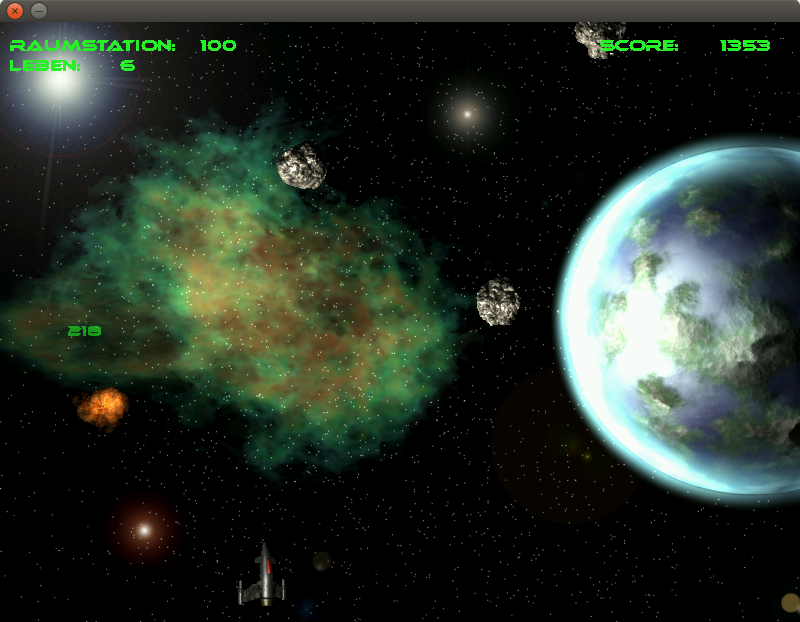
\includegraphics[width=\linewidth]{game3.png}
 \label{fig:game}
 \caption{2d space game}
\end{figure}

\subsection{Problem Statement}

Before the start of this capstone project the game existed only as an interactive, GUI-based game playable using the keyboard. 
The first task was therefore not concerned with machine learning but with software engineering:
The program had to be modularized to allow for a learning algorithm to use the game logic that is used when a human plays it.
Special attention needed to be paid to the time that passes between two frames:
As usual, a target number of frames per second was set.
In every iteration of the main loop the game logic is applied: It moves the elements of the game according to the time that has passed since the last frame which is supposed to be 1/60th of a second.
Afterwards, GUI elements are drawn on the screen and the thread then sleeps until it is time for the next iteration for .
The same needed to be true when training the algorithm without a GUI.
Hence, a fake timer was implemented that always said the time between frames was 1/60th of a second.
This way, the algorithm could be trained without a GUI in much shorter time and the results would be applicable later even in a GUI run.

% Erklären, woraus das Spiel besteht (Spawnraten, Geschwindigkeiten etc).
% Erklären, auf welcher Basis gelernt wird (keine Bilder, sondern Daten)
The problem statement for the machine learning part of this project is a little more intricate.
Nowadays, reinforcement learning algorithms combined with convolutional neural networks are powerful enough to learn games only from sensory input\cite{DeepmindBreakout}.
Thus, a decision had to be made regarding what information to give to the algorithm:
It could either use the actual data the game logic works with or the visual representation of this data.
However, since this project is not supposed to compete with a Google project - neither regarding manpower nor computational ressources - the decision was made to use the data that is already there:

\begin{itemize}
 \item Lives left: Every time the space ship gets hit by an asteroid, the player will lose a life and eventually the entire game if no lives are left. The player starts with six lives.
 \item Space station health: Every time an asteroid is allowed to cross the screen, the space station will lose 16 health points and regenerate it at a fixed rate of five points per second until it is back at 100 again. If the space station health drops below $0$, the player will lose the game.
 \item Asteroids: Set of x- and y-coordinates describing the positions of the asteroids
 \item Ship position: The ship can move left and right on the lower edge of the screen
 \item Weapons array cooldown: $0.5$ seconds need to have passed between shots.
 \item Shot positions: Set of x- and y-coordinates of the shots the player has already fired.
\end{itemize}

After specifying the data the algorithm can work on we can now define the task at hand using the insights from \cite{712192}:

In each frame the algorithm is presented with the data explained above - the so called \emph{state} of the game - and has to make a decision what to do next - taking a so called \emph{action}.
To do so, we need to find a deterministic policy $\pi$ that yields an action $a$ for every given state $s$:
\[\pi(s)=a\]
However, we do not just want to find \emph{any} such policy, we want to find one that maximizes the score before the game is over. 
Therefore, we define a value function $V$ so that
\[V_\pi(s) = E[R] = E[\sum_{t=0}^\infty\gamma^tr_t|s_0=s]\].
$R$ is the expected return following policy $\pi$ starting in state $s$.
Two more things are needed to fully grasp this formula: The reward $r_t$ and the discount factor $\gamma$.
The former is the direct return for an action given by the environment and can be positive or negative.
The later is a value between $0$ and $1$ and determines how strongly future rewards are taken into account.

The task to solve in this setting is to find a policy $\pi$ which maximizes $V^\pi(s)$:
\[V^*(s) = \max_\pi V^\pi(s)\]
Since we cannot know the number of policies it is computationally unfeasable to directly calculate the optimal policy.

Hence, an algorithm is needed that can approximate the optimal policy in an iterative fashion.
It will start with an initial guess at the optimal policy and slowly improve its performance until it converges.

% In this section, you will want to clearly define the problem that you are trying to solve, including the strategy (outline of tasks) you will use to achieve the desired solution.
% You should also thoroughly discuss what the intended solution will be for this problem. Questions to ask yourself when writing this section:

% Is the problem statement clearly defined? Will the reader understand what you are expecting to solve?
% Have you thoroughly discussed how you will attempt to solve the problem?
% Is an anticipated solution clearly defined? Will the reader understand what results you are looking for?

% It might therefore be wise to crash the ship into an asteroid if it cannot be stopped otherwise and the space station is at low health.
% In other situations it could be beneficial to let the asteroids hit the space station, since its health bar is still full.

% The task of this project is therefore to let a machine learning algorithm figure out how to achieve the highest score.
% In order not to bias the learning agent, no human-devised strategies will be programmed into the approach.
% This will lead to an algorithm that potentially uses methods a human would not have thought of and that can cope with any of the random situations, the game throws at it.

\subsection{Metrics}
% In this section, you will need to clearly define the metrics or calculations you will use to measure performance of a model or result in your project. 
%These calculations and metrics should be justified based on the characteristics of the problem and problem domain. Questions to ask yourself when writing this section:

% Are the metrics you’ve chosen to measure the performance of your models clearly discussed and defined?
% Have you provided reasonable justification for the metrics chosen based on the problem and solution?
In contrast to supervised learning problems where you can easily measure the performance using precision, recall or F-scores, the performance of the proposed algorithm is only measurable using feature offered by the application domain.
Since the task of the algorithm is to maximize the score, that is the measurement we are going to use.
The algorithm will first train by playing the game until it has explored the state space sufficiently and has exploited the gained knowledge to optimize the policy.
To make the analysis of the performance statistically sounder, the algorithm will then be tested $100$ times and we will take note of the minimum and maximum score as well as the mean and standard deviation.
\section{Analysis}
% (approx. 2-4 pages)

\subsection{Data Exploration}
\label{dataexploration}
% In this section, you will be expected to analyze the data you are using for the problem. This data can either be in the form of a dataset (or datasets), input data (or input files), or even an environment.
%The type of data should be thoroughly described and, if possible, have basic statistics and information presented (such as discussion of input features or defining characteristics about the input or environment). 
%Any abnormalities or interesting qualities about the data that may need to be addressed have been identified (such as features that need to be transformed or the possibility of outliers). Questions to ask yourself when writing this section:

% If a dataset is present for this problem, have you thoroughly discussed certain features about the dataset? Has a data sample been provided to the reader?
% If a dataset is present for this problem, are statistics about the dataset calculated and reported? Have any relevant results from this calculation been discussed?
% If a dataset is not present for this problem, has discussion been made about the input space or input data for your problem?
% Are there any abnormalities or characteristics about the input space or dataset that need to be addressed? (categorical variables, missing values, outliers, etc.)
As described in the problem statement, there is no datasat to analyze.
Rather, the game consists of several elements relevant to the game logic that make up the state space.
In detail, these are:

\begin{itemize}
 \item Player lives: As described above, this is an integer ranging from $6$ to $0$.
 \item Space station health: As described above, this is an integer ranging from $100$ to $0$.
 \item Asteroids: The asteroids spawn at eight equidistant points off the top edge of the screen. The spawnpoint is chosen at random. In every subsequent frame they travel with a speed of 200 pixels per second towards the lower edge of the screen. Thus, in each frame there is a set of (x,y) coordinates describing where the asteroids are. Each asteroid is 64 pixels wide and 64 pixels high.
 \item Ship position: The player can be at any point on the lower corner of the screen as long as he does not crash into the border of the screen.
 \item Weapons array cooldown: A floating point number keeping track of how long ago the last shot was fired. The player can only fire if the last shot was more than half a second ago.
 \item Shot position: When the player shoots, a shot spawns at the ship's position and travels up in a vertical line with a speed of $400$ pixels per second until it hits an asteroid or eventually goes off screen and gets deleted.
\end{itemize}
Furthermore, there are details to the game logic that are not directly observable and that don't change over time:
\begin{itemize}
 \item The speeds the player and the asteroids travel at which is 300 and 200 pixels per second respectively.
 \item The amount of health the space station loses when getting hit by an asteroid, here: 16 health points per hit.
 \item The rate at which the space station gets repaired, here: One health point every $0.35$.
 \item The rate at which the asteroids spawn, here: One every $0.75$ seconds.
 \item The size of the screen is 800 by 600 pixels.
\end{itemize}

Since this second set of information is not directly conveyed to the human player either, it is not supposed to enter into the state space.
We will therefore focus on how the first set of information forms the state space and make a guess at how large it is to estimate the difficulty of the task at hand.

The combination of the player's lives and space station health brings the state space to a size of $7 \cdot 101 = 707$.

The combinations of asteroids are a little harder to calculate: They spawn every $0.75$ seconds and need $\frac{600}{200} = 3$ seconds to travel to the bottom of the screen.
Since they spawn a little above the screen - at a y-position of $-60$ -  and crash into the space station at y-position $590$, there can be at maximum five asteroids at once.
% If we limit the coordinates to integers, the position of one asteroid can take one of $600 \dot 8 = 4800$ values.
Since there is a $0.75$ pause between asteroids, the cardinality is not just the amount of different positions an asteroid can be in to the power of five.
If there are five asteroids, the one that spawned earliest is at least at y-position $540$: It spawned at $-60$, then three seconds passed making it travel to $540$ and making four more asteroids spawned during that time.
The first asteroid can be in $(590-540)\cdot8 = 400$ positions.
The y-positions of every subsequent asteroid is irrelevant since it is directly dependent on the first asteroids y-positions.
Therefore, only their x-positions matter.
This brings the state space spanned by the asteroids to $400\cdot8\cdot8\cdot8\cdot8 = 1,638,400$ different combinations.

The ships position ranges from $0$ to $752$\footnote{This is a programming error. It should only be able to fly to an x-position of $736$, because it is $64$ pixels wide. However, in a previous version of the game, the sprite for the ship was $48$ by $48$ pixels and the maximum x-position was never changed after.}.

The weapons array cooldown is a floating point number that can in theory take any positive value.
However, if we assume that the player fires a shot at the latest one second after the last shot was fired - so half a second after he is already eligible to fire another shot - we can limit the combinations to $60$, because there are $60$ frames in a second.

A shot can - in principal - be in any position of the screen, as long as it does not overlap with an asteroid.
Since a shot travel $400$ pixels per second and two shots can be taken per second, there can be three shots at the same time.
Each can roughly be at $200 \cdot 600 = 120000$ positions, bringing the combinations in total to a staggering number of $1728000000000000$.

This leads to a total size of the state space of $7\cdot101\cdot1638400\cdot753\cdot60\cdot(600\cdot200)^3 = 90,433,495,498,752,000,000,000,000,000L = 90E27$.

Obiviously, this is much too big to be handled in a project of this scope, making it crucial to find a way to reduce the size of the state space without losing too much information or biasing the algorithm.
How this is achieved will be explained in the chapter \nameref{datapreprocessing}.


\subsection{Exploratory Visualization}
% In this section, you will need to provide some form of visualization that summarizes or extracts a relevant characteristic or feature about the data. 
%The visualization should adequately support the data being used. Discuss why this visualization was chosen and how it is relevant. Questions to ask yourself when writing this section:

% Have you visualized a relevant characteristic or feature about the dataset or input data?
% Is the visualization thoroughly analyzed and discussed?
% If a plot is provided, are the axes, title, and datum clearly defined?
Since this project is about a game, every frame of the game is a visualization of the data we are to examine.
Therefore, the example screenshot \ref{fig:game} will be analyzed.
We can see that there are three asteroids which spawned in the middle region of the screen.
The vertical distance between them is the same since they spawned at a fixed interval.
One asteroid was shot down recently: The explosion caused by that is still visible and it yielded a score of 218.
The player and the space station are both still at full health and the player has reached a score of 1353 points so far.
\subsection{Algorithms and Techniques}
% In this section, you will need to discuss the algorithms and techniques you intend to use for solving the problem. 
% You should justify the use of each one based on the characteristics of the problem and the problem domain. Questions to ask yourself when writing this section:

% Are the algorithms you will use, including any default variables/parameters in the project clearly defined?
% Are the techniques to be used thoroughly discussed and justified?
% Is it made clear how the input data or datasets will be handled by the algorithms and techniques chosen?


\subsection{Benchmark}
% In this section, you will need to provide a clearly defined benchmark result or threshold for comparing across performances obtained by your solution.
% The reasoning behind the benchmark (in the case where it is not an established result) should be discussed. Questions to ask yourself when writing this section:

% Has some result or value been provided that acts as a benchmark for measuring performance?
% Is it clear how this result or value was obtained (whether by data or by hypothesis)?

Since the task of the agent is to maximize the score and there is no ground truth to what it can and should achieve, we can only compare it to the performance of other players:
Human players will be asked to play the game to the best of their ability.
We will take note of the statistical properties of the scores they achieve the same way we do for the trained player.
However, in order to save time, human players will not be asked to play $100$ times: $5$ runs will have to suffice.
Furthermore, a random agent will play the game in order to find a bottom line for the score count.
The proposed system will be compared to these players and is expected to perform much better than the random player and hopefully as good as humans or even better.
\section{Methodology}
% (approx. 3-5 pages)

\subsection{Data Preprocessing}
\label{datapreprocessing}
% In this section, all of your preprocessing steps will need to be clearly documented, if any were necessary. 
% From the previous section, any of the abnormalities or characteristics that you identified about the dataset will be addressed and corrected here. Questions to ask yourself when writing this section:

% If the algorithms chosen require preprocessing steps like feature selection or feature transformations, have they been properly documented?
% Based on the Data Exploration section, if there were abnormalities or characteristics that needed to be addressed, have they been properly corrected?
% If no preprocessing is needed, has it been made clear why?
As discussed in the chapter \nameref{dataexploration} the state space of the game is too large to let a computer agent draw knowledge from it.
The need for computational power and storage would both exceed the scope of this project by far.
Furthermore, the true state space is probably a subspace of what was explained above with much fewer dimensions.
\emph{True state space} here means the space that needs to be explored in order to achieve a reasonable performance. 
The distinction between many states in the original state space does not yield any knowledge that can be exploited.
Here are a few examples to highlight this:
\begin{itemize}
 \item If a shot is going to travel off screen without a chance of hitting another asteroid because it will leave the game before the asteroid can spawn, the position of that shot does not matter at all.
 \item If an asteroid is too far away from the ship in the x-axis and will hit the space station regardless of what the player does, the position of that asteroid also does not matter.
\end{itemize}
These were examples for information that makes not difference at all.
There is more information that can probably be summarized: We will lose a bit of information, but the increase in performance due to the reduction of the problem's dimensionality might compensate for that:
\begin{itemize}
 \item The exact number of the space station's health points will be quantized into four categories: $0$ HP, $1$ to $33$ HP, $34$ to$ 67$ HP and more than $68$ HP
 \item The asteroids positions will be boiled down to one piece of information: Where is the asteroid will not get hit by a shot so far and that is still reachable for the player? 
 This is stored in using two bits: It might be to the left, to the right, in front of the ship or non-existent.
 \item The possibly $60$ state of the weapons array will be expressed in one bit: Is it possible to shoot or not?
 \item The player's position will take two bits: Can the ship move left, right or both?
\end{itemize}




\subsection{Implementation}
% In this section, the process for which metrics, algorithms, and techniques that you implemented for the given data will need to be clearly documented. It should be abundantly clear how the implementation was carried out, and discussion should be made regarding any complications that occurred during this process. Questions to ask yourself when writing this section:

% Is it made clear how the algorithms and techniques were implemented with the given datasets or input data?
% Were there any complications with the original metrics or techniques that required changing prior to acquiring a solution?
% Was there any part of the coding process (e.g., writing complicated functions) that should be documented?
\subsection{Refinement}
% In this section, you will need to discuss the process of improvement you made upon the algorithms and techniques you used in your implementation. For example, adjusting parameters for certain models to acquire improved solutions would fall under the refinement category. Your initial and final solutions should be reported, as well as any significant intermediate results as necessary. Questions to ask yourself when writing this section:

% Has an initial solution been found and clearly reported?
% Is the process of improvement clearly documented, such as what techniques were used?
% Are intermediate and final solutions clearly reported as the process is improved?
\section{Results}
% (approx. 2-3 pages)

\subsection{Model Evaluation and Validation}
% In this section, the final model and any supporting qualities should be evaluated in detail. It should be clear how the final model was derived and why this model was chosen. In addition, some type of analysis should be used to validate the robustness of this model and its solution, such as manipulating the input data or environment to see how the model’s solution is affected (this is called sensitivity analysis). Questions to ask yourself when writing this section:

% Is the final model reasonable and aligning with solution expectations? Are the final parameters of the model appropriate?
% Has the final model been tested with various inputs to evaluate whether the model generalizes well to unseen data?
% Is the model robust enough for the problem? Do small perturbations (changes) in training data or the input space greatly affect the results?
% Can results found from the model be trusted?
\subsection{Justification}
% In this section, your model’s final solution and its results should be compared to the benchmark you established earlier in the project using some type of statistical analysis. You should also justify whether these results and the solution are significant enough to have solved the problem posed in the project. Questions to ask yourself when writing this section:

% Are the final results found stronger than the benchmark result reported earlier?
% Have you thoroughly analyzed and discussed the final solution?
% Is the final solution significant enough to have solved the problem?
\section{Conclusion}
% (approx. 1-2 pages)

\subsection{Free-Form Visualization}
% In this section, you will need to provide some form of visualization that emphasizes an important quality about the project. It is much more free-form, but should reasonably support a significant result or characteristic about the problem that you want to discuss. Questions to ask yourself when writing this section:

% Have you visualized a relevant or important quality about the problem, dataset, input data, or results?
% Is the visualization thoroughly analyzed and discussed?
% If a plot is provided, are the axes, title, and datum clearly defined?
\subsection{Reflection}
% In this section, you will summarize the entire end-to-end problem solution and discuss one or two particular aspects of the project you found interesting or difficult. You are expected to reflect on the project as a whole to show that you have a firm understanding of the entire process employed in your work. Questions to ask yourself when writing this section:

% Have you thoroughly summarized the entire process you used for this project?
% Were there any interesting aspects of the project?
% Were there any difficult aspects of the project?
% Does the final model and solution fit your expectations for the problem, and should it be used in a general setting to solve these types of problems?
\subsection{Improvement}
% In this section, you will need to provide discussion as to how one aspect of the implementation you designed could be improved. As an example, consider ways your implementation can be made more general, and what would need to be modified. You do not need to make this improvement, but the potential solutions resulting from these changes are considered and compared/contrasted to your current solution. Questions to ask yourself when writing this section:

% Are there further improvements that could be made on the algorithms or techniques you used in this project?
% Were there algorithms or techniques you researched that you did not know how to implement, but would consider using if you knew how?
% If you used your final solution as the new benchmark, do you think an even better solution exists?



\bibliographystyle{plain}
\bibliography{bib}
\end{document}
